%!TEX root = ../../../adrien_gomar_phd.tex

To assess the capability of the HB operator that will be used in the present work 
defined in Eq.~\eqref{eq:sm_hb_mono_source_term_matrix} to
provide accurate approximations of the time-derivative, 
we consider the simple example of a pure
five-harmonic signal of the form:
\begin{equation}
    \label{eq:sum_sin}
    u(t) = \cos(\omega t) + \sin(2 \omega t) +
    \cos(3 \omega t) + \sin(4 \omega t) + \cos(5 \omega t),
\end{equation}
where $\omega = 2 \pi f$ and $f$ is the temporal frequency of
the considered phenomenon.
The analytical derivative is then:
\begin{equation}
    \label{eq:sum_sin_deriv}
    \frac{\partial u}{\partial t} = 
    \omega\left[ -\sin(\omega t) + 
    2\cos(2 \omega t) -
    3\sin(3 \omega t) + 
    4\cos(4 \omega t) -
    5\sin(5 \omega t)\right].
\end{equation}
The exact derivative is compared to the approximated derivative by applying 
the HB operator defined in Eq.~\eqref{eq:sm_hb_mono_source_term_matrix}
and two different Finite-Difference (FD) schemes,
a second-order centered scheme:
\begin{equation}
    \frac{\partial u}{\partial t} (t=t_q) \approx 
    \frac{u^{q+1} - u^{q-1}}{2 \Delta t},
    \label{eq:hb_op_center2}
\end{equation}
and a fourth-order centered scheme:
\begin{equation}
    \frac{\partial u}{\partial t} (t=t_q) \approx 
    \frac{-u^{q+2} + 8 u^{q+1} - 8 u^{q-1} + u^{q-2}}{12\Delta t}.
    \label{eq:hb_op_center4}
\end{equation}

For finite-difference schemes, 
we assume that the time line is discretized 
by a regular mesh of step $\Delta t$, such that $t_q = q \Delta t$.
Figure~\ref{fig:hb_operator_sample} shows the resulting approximations 
of the derivative over one period.
\begin{figure}[htb]
  \centering
  \subfigure[HB]{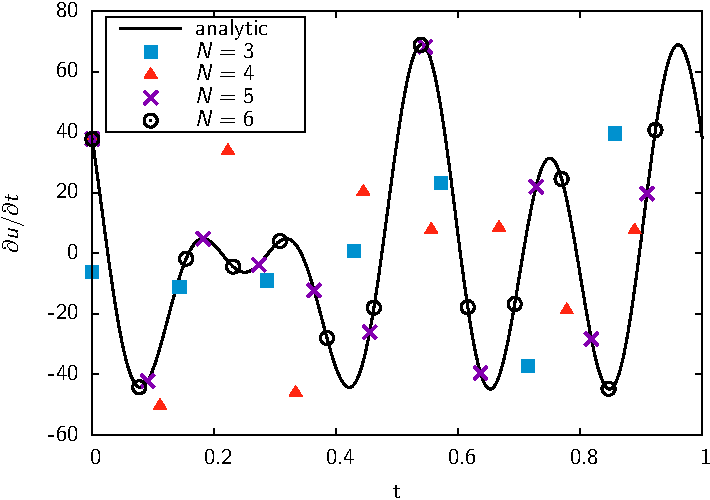
\includegraphics[width=.4\textwidth]{HB_OPERATOR_PPT_HB.pdf}}
  \subfigure[FD 2\textsuperscript{nd} order]{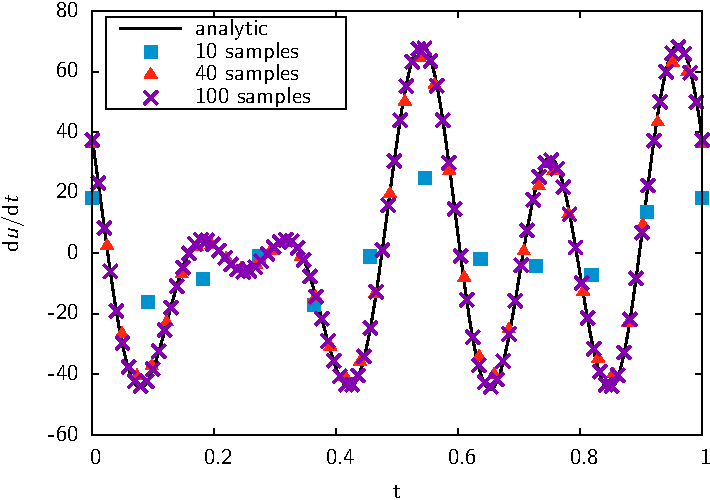
\includegraphics[width=.4\textwidth]{HB_OPERATOR_PPT_FD2.pdf}}
  \subfigure[FD 4\textsuperscript{th} order]{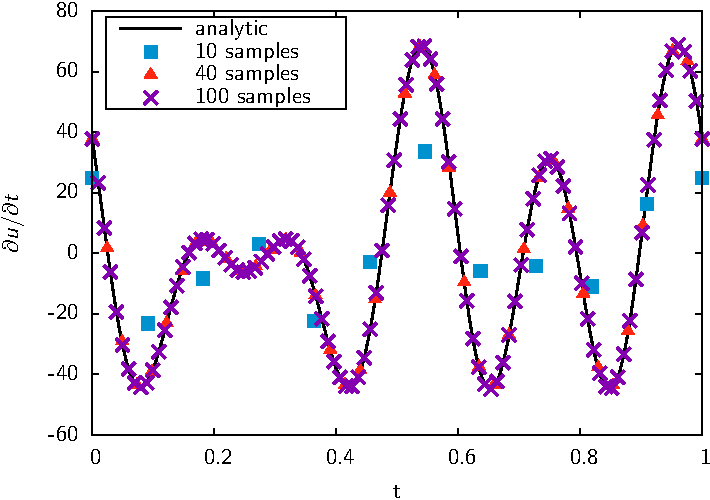
\includegraphics[width=.4\textwidth]{HB_OPERATOR_PPT_FD4.pdf}}
  \caption{Time-derivative estimation by the harmonic balance operator,
  the 2\textsuperscript{nd} order and 4\textsuperscript{th} finite-difference schemes.}
  \label{fig:hb_operator_sample}
\end{figure}
Four sampling levels
are tested for the HB operator: 7, 9, 11 and 13~time instances per period
corresponding to, respectively, $N=3$, 4, 5 and 6.
For the FD schemes, the periodicity time interval is sampled by
10, 40 and 100 points.
As expected, the error of the 4\textsuperscript{th}~order FD
decreases faster  than the 2\textsuperscript{nd}~order for a given sampling level.
For 40~samples, the 4\textsuperscript{th} order FD
scheme almost fits the analytical solution. On the other-hand,
the HB operator prediction is superimposed with the analytical solution
by using 11~samples, i.e. $N=5$. Beyond that, further increasing the
number of harmonics (or samples)
does not improve the solution.

To quantitatively analyze the results, the 
$\mathcal{L}_2$-norm of the absolute error with respect to the analytical
derivative is computed for the different schemes and 
sampling levels (see Fig.~\ref{fig:hb_operator_error}).
\begin{figure}[htb]
  \centering
   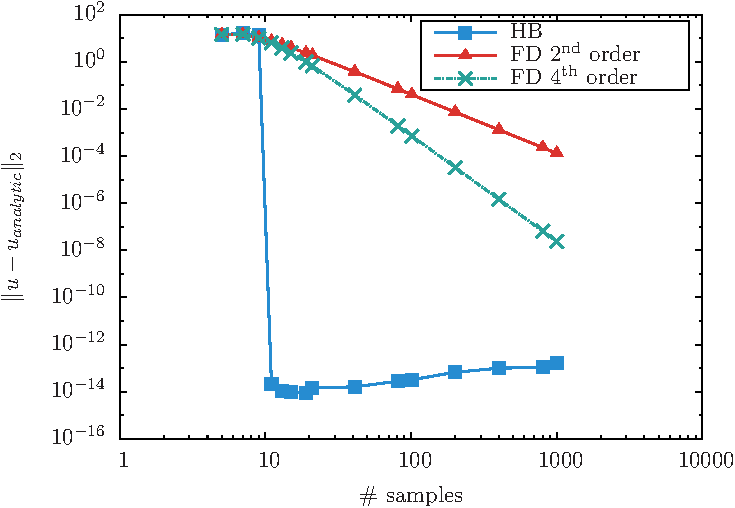
\includegraphics[width=.55\textwidth]{HB_OPERATOR_ERROR.pdf}
   \caption{$\mathcal{L}_2$-norm of the error for each time-derivative
   schemes.}
  \label{fig:hb_operator_error}
\end{figure}
When the number of harmonics is low 
(i.e. $N < 5$), the error is high as Fig.~\ref{fig:hb_operator_sample}
suggests. But as soon as $N \geq 5$, the error
drastically decreases to machine precision.
This illustrates the spectral accuracy as explained in 
Sec.~\ref{sec:spectral_accuracy}. In fact, the function defined
in Eq.~\eqref{eq:sum_sin_deriv} approximated by the spectral operator
is infinitely differentiable and periodic in $[0, T]$.
Thus, using the properties established in Sec.~\ref{sec:spectral_accuracy},
the convergence rate of the spectral operator is $\mathcal{O} (k^{-\infty})$
for $k > k_0$, here $k_0=5$. In this case, $k_0$
reflects the frequency content of the signal (namely $5$ harmonics).
% This simple example shows that the accuracy of the 
% harmonic balance operator strongly depends on the frequency 
% content of the time signal and on its sampling. 
% This is further investigated in the following.